\newpage
\chapter{Пересечения фрактальных кубов}


\section{Предварительные сведения}

\begin{definition}
[Olsen L. (1998); Lau K., Luo J.J.,Rao H. (2013)]
Пусть  $D=\{d_1,\ldots,d_r\},\; d_i\in\{0,1,\ldots,n-1\}^k$, где $n\ge 2$, а $1<\#D<n^k$.\\
{\em Фрактальным $k$-кубом} порядка $n$ с {\em множеством единиц $D$} называют компактное множество $K\IN\rr^k$, удовлетворяющее $$K=\dfrac{K+D}{n}$$
\end{definition}

\begin{figure}[H]
    \centering
    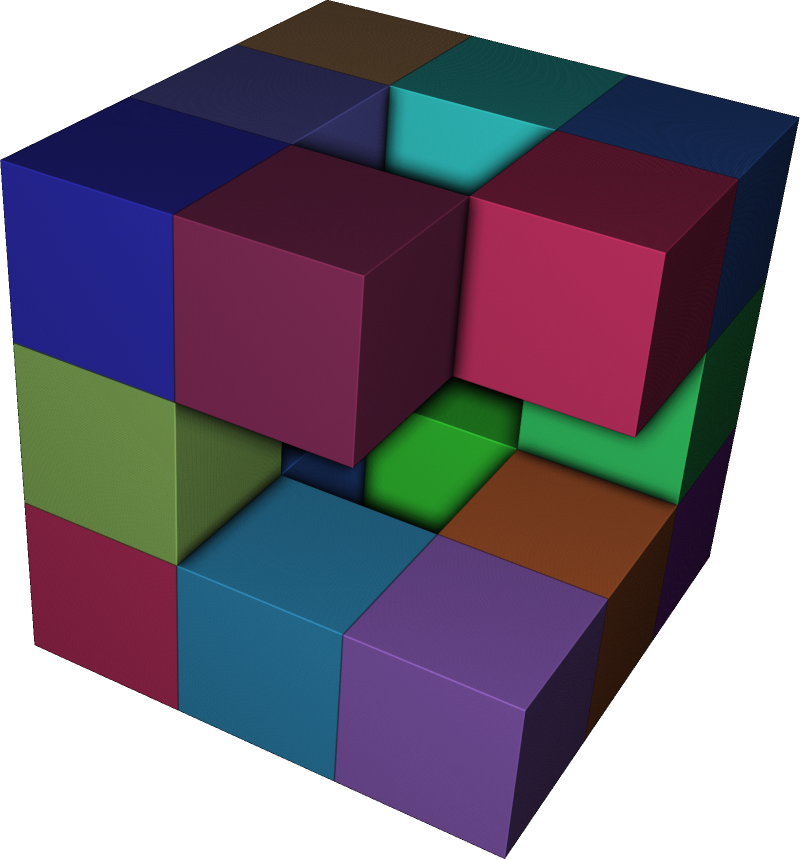
\includegraphics[width=0.45\textwidth]{FQD.png}
    \hfill
    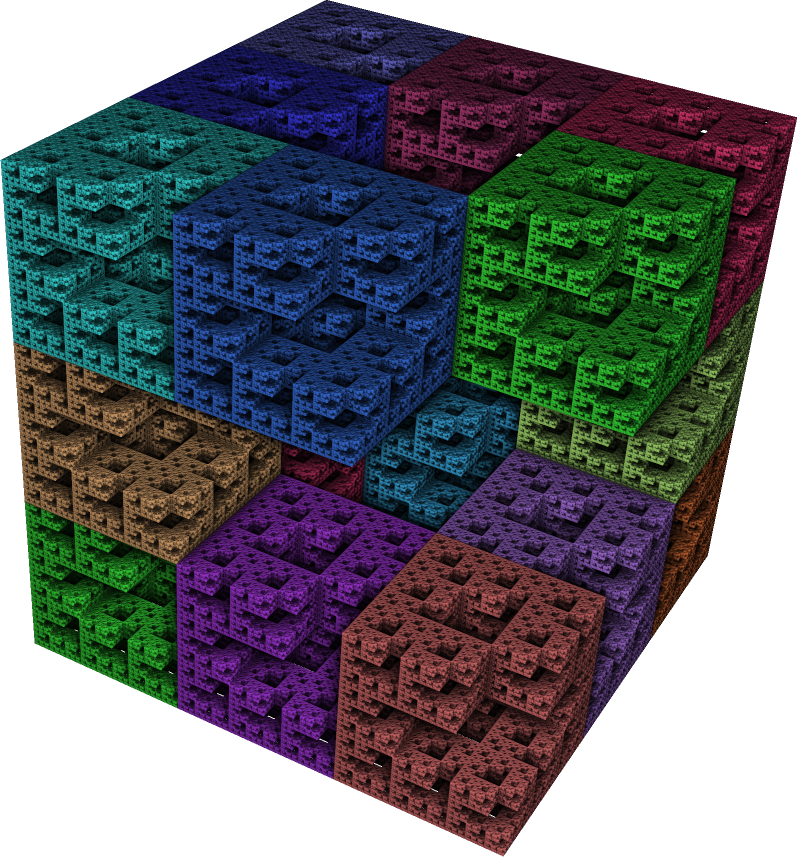
\includegraphics[width=0.45\textwidth]{FQK.png}
    \caption{Фрактальный куб}
    % \label{fig:enter-label}
\end{figure}

В случаях, когда $k=1$, $k=2$ и $k=3$, мы называем $K$  \emph{фрактальным отрезком}, \emph{фрактальным квадратом} и \emph{фрактальным кубом} сответственно.

\begin{remark}
Фрактальный $k$-куб $K=\dfrac{K+D}{n}$ с множеством единиц $D=\{0,1,\ldots,n-1\}^k$ есть единичный $k$-мерный куб $P^k$.
\end{remark}

Из этого можно сделать естественный вывод о том, что любой фрактальный $k$-куб $K$ содержится в единичном $k$-мерном кубе $P^k$ как его податтрактор.
 
% Слегка злоупотребляя терминологией, мы иногда будем называть изометрические изображения фрактального $k$-куба тем же именем.


\section{Единичный $k$-куб, его грани и сечения} 
 
\subsection{Семейство граней единичного куба} 

Каждый фрактальный $k$-куб является подмножеством единичного $k$-куба $P^k$ в $\rr^k$, поэтому мы вводим некоторые обозначения, связанные с границей, гранями и сечениями единичного куба $P^k$.

Обозначим через $A_k$ множество $\{-1,0,1\}^k$. 
Существует естественное взаимно однозначное соответствие между семейством всех граней куба $P^k$ и множеством $A_k$.
Чтобы установить это, мы рассмотрим центр $(1/2,\ldots,1/2)$ куба $P^k$, который мы обозначим как $c$.
Каждому вектору $\bma=(\al_1,\ldots\al_k)\in A_k$ мы ставим в соответствие единственную грань $P_\bma$ куба $P^k$, центром которого является $c_\bma=c+\bma/2$, и наоборот. 
Противоположный вектор $-\bma$ определяет грань $P_{-\bma}$ с центром $c_{-\bma}=c-\bma/2$, которая параллельна и противоположна грани $P_{\bma}$, и следовательно, $P_{-\bma}+\bma=P_\bma$. 

 
\begin{figure}[H]
    \centering
    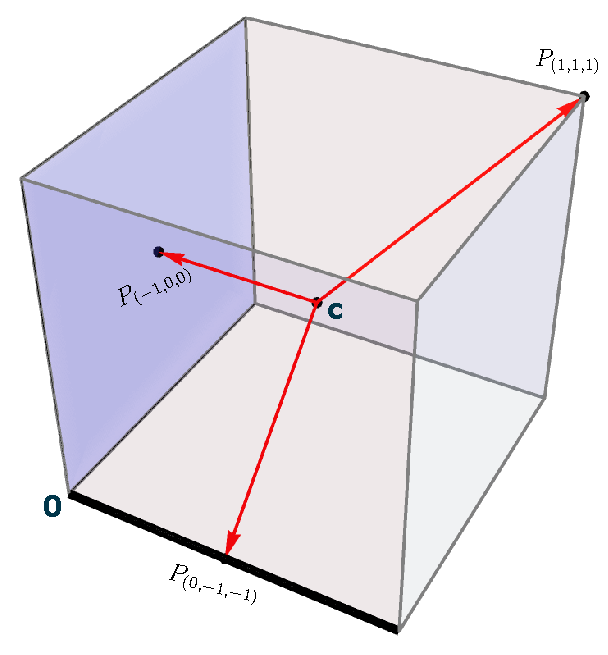
\includegraphics[width=0.42\textwidth]{faces.pdf}
    \hspace{0.05\textwidth}
    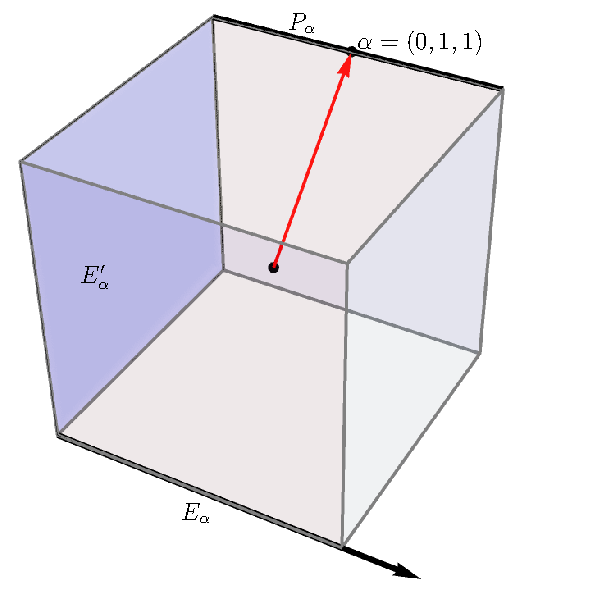
\includegraphics[width=0.47\textwidth]{faces3.pdf}
    \caption{Грани $P_\bma$ единичного (слева) и подпространства $E_\bma$ и $E'_\bma$ (срава)}
    \label{fig:uq_faces}
\end{figure}

Равенство $P_{-\bma}+\bma=P_\bma$ показывает, что кубы $P^k$ и $P^k+\bma$ пересекаются по своей общей грани. 
Эта общая грань является гранью $P_\bma$ куба $P^k$, и также гранью $P_{-\bma}+\bma$ куба $P^k +\bma$.


\subsection{Связь между гранями и подпространствами.} 

Для каждого $\bma\in A_k$ множества $J_\bma=\{i:\al_i=0\}$ и $J'_\bma=\{i:|\al_i|= 1\}$ порождают ортогональные комплементарные подпространства $E_\bma=\operatorname{span}\{e_i, i\in J_\bma\}$ и $E'_\bma=\operatorname{span}\{e_i, i\in J'_\bma\}$.
Отсюда следует, что $\bma\in E'_\bma$ и что грань $P_\bma$ параллельна подпространству $E_\bma$.
Мы также определяем грань $P'_\bma=P\cap E'_\bma$, которая является единственной гранью, дополняющей $P_\bma$ и содержащей начало координат.
Мы обозначим ортогональные проекции $\rr^k$ на $E_\bma$ через $\pr_{\bma}$ и на $E'_\bma$ через $\pr'_{\bma}$.
 
Определив $|\bma|=(|\al_1|+\ldots +|\al_k|)$ можно заметить, что размерности подпространств $E_\bma$ и $E '_\bma$ равны $j_\bma=k-|\bma|$ и $j_\bma'=|\bma|$ соответственно.
  
Заметим, что все грани $P_\bma$, для которых множество $J_\bma$ одинаково, являются изометрическими и параллельными.
Поскольку каждое ненулевое $\al_i$ равно $+1$ или $-1$, то существует $2^{|\bma|}$ различных вектора $\bmb\in A_k$, для которых $J_\bmb=J_\bma$.
Для любого вектора $\bmb\in A_k$ равенство $J_\bmb=J_\bma$ подразумевает равенства $E_\bmb=E_\bma$, $E'_\bmb=E'_\bma$, $P'_\bmb=P'_\bma$, а также соответствующие равенства для проекций $\pr_\bmb, \pr'_\bmb$ и размерностей $j_\bmb$ и $j'_\bmb$.
Все они зависят только от $J_\bma$.
 

Всякий раз, когда известно, о каком $\bma$ идет речь, мы будем писать $J, J', \pr, \pr', j$ и $j'$ опуская нижний индекс $\bma$.
 
\begin{definition}\label{INperp}
Для $\bma,\bmb\in A_k$ мы записываем $\bma\sqsubseteq\bmb$, если для любого $i\in J'_\bma$, $\al_i=\be_i$ или, что эквивалентно, $J'_\bma\subseteq J'_\bmb$.
Если $J'_\bma\cap J'_\bmb=\0$, мы говорим, что $\bma$ и $\bmb$ являются взаимодополняющими и пишем $\bma\perp\bmb$.
Мы обозначим через $A_\bma$ множество всех $\bmb\in A$, дополняющих $\bma$.
\end{definition}

Если $\bmb=\bma+\bmg$ является суммой взаимодополняющих ненулевых векторов, то $\bma\sqsubset\bmb$.
И наоборот, если $\bma\sqsubset\bmb$, то вектор $\bmg=\bmb-\bma$ также является элементом $A_k$, а значит $\bmg\perp\bma$.


Если $\bma\bot\bmb$, то подпространства $E'_\bma$ и $E'_\bmb$ ортогональны и $E'_\bma\cap E'_\bmb =\{0\}$. 
Следовательно, $E'_\bma\IN E_\bmb$ и $E'_\bmb\IN E_\bma$.

Если $\bma\bot\bmb$, то $P_{\bma+\bmb}=P_\bma\cap P_\bmb$.

Вектор $\bma\in A_k$ максимален относительно отношения $\sqsubset$ тогда и только тогда, когда $J_\bma=\0$. 
В этом случае $P_\bma=\{c+\bma/2\}$ является вершиной куба $P^k$.


 
\subsection{Грани, содержащие начало координат.}  
Мы обозначим через $P^0_{\bma}=P^k\cap E_\bma$ грань, которая параллельна $P_\bma$ и содержит начало координат.
Вектор  $\bma^0$, который параллельно переносит $P^0_{\bma}$ в $P_\bma$, содержит координаты $\bma_i^0=\max\{\max_i,0\}$ для любых $i=1,\ldots,k$.
Вектор $(-\bma)^0$, который параллельно переносит $P^0_{\bma}$ в $P_{-\bma}$, равен $(-\bma)^0=\bma^0-\bma.$
Таким образом, $P_\bma=\bma^0 +P^0_{\bma}$ и $P_{-\bma}=\bma^0-\bma+P^0_{\bma}$.

Дополнительная грань $P'_\bma=E'_\bma\cap P$ содержит начало координат по своему определению.

Если $\bma\bot\bmb$, то $P^0_{\bma+\bmb}=P^0_\bma\cap P^0_\bmb=P_\bma\cap P_\bmb-\bma^0-\bmb^0$.

Если $P_\bma$ является вершиной куба $P^k$, то $P^0_\bma=\{\bm{0}\}$ является вершиной в начале координат.
 
 
\subsection {Граница единичного куба $P^k$ и его грани.} 

Поскольку $P_\bma=P^k\cap(\bma+P^k)$, то множество
$\{\bma+P^k, \bma\in A\mmm \{0\}\}$ --- это множество всех соседей $P ^ k$ в семействе $\{d+P^k, d\in\zz^k\}$, а граница $P^k$ представлена формулой 
\begin{equation}\label{dpk}
\dd P^k=\bigcup\limits_{\bma\in A_k\mmm \{0\}}P_\bma
\end{equation}
 
Аналогично, для каждого $\bma\in A$ граница $P_\bma$ представлена следующим выражением
 
\begin{equation}\label{dpal}
    \dd P_\bma= \bigcup\limits_{\bmb\sqsupset\bma}P_{\bmb}=\bigcup\limits_{\bmg\in A_\bma\mmm\{0\}}P_{\bma+\bmg}
\end{equation}

С учётом равенств $P_\bma=\bma^0+P^0_{\bma}$ и $P_{\bma+\bmb}= P^0_{\bma+\bmb}+\bma^0+\bmb^0$, мы получим аналогичную формулу и для $\dd P^0_\bma$:

\begin{equation}\label{dpa0}
    \dd P^0_\bma=\bigcup\limits_{\bmb\in A_\bma\mmm\{0\}}P^0_{\bma+\bmb}+\bmb^0.
\end{equation}


\section{Проекции, сечения, грани и $p$-е измельчение фрактального $k$-куба $K$.}

В этом разделе мы докажем, что проекция фрактального куба $K$ на грань $P_\bma$ и пересечение $K_\bma=P_\bma\cap K$ являются фрактальными кубами.

\subsection{Проекции и $\al$-сечения фрактального куба.}

 
Пусть $K\IN P^k$ --- фрактальный $k$-куб порядка $n$ с множеством единиц $D\IN \{0,1,\ldots,n-1\}^k$.
Учитывая $d_i\in \{0,1,\ldots,n-1\}^k$, обозначим $S_i(x)=\dfrac{x+d_i}{n}$ и $S_{i_1\ldots i_p}=S_{i_1}\cdot\ldots \cdot S_{i_p}$.

Фиксированной точкой отображения $S_i$ является $\dfrac{d_i}{n-1}$. Она будет обозначаться как $c_i$.


\begin{lemma}\label{lem1}
Для любого $\bma\in A_k$ проекция $\pr'_{\bma}(K)$ представляет собой фрактальный куб с множеством единиц $\pr'_{\bma}(D)$.
\end{lemma}

\begin{proof} Очевидно, что
$\pr'_\bma(K)=\pr'_{\bma}\dfrac{K+D}{n}=\dfrac{\pr'_\bma(K) +\pr'_{\bma}(D)}{n}$.   
\end{proof}

\begin{proposition}\label{c0inK}
Пусть $d_{i_1},\ldots  ,d_{i_p},d_0\in I^k$ и
$c_0={d_0}/({n-1})$.
Тогда $c_0\in S_{i_1\ldots i_p}(P)$ тогда и только тогда, когда все $d_{i_j}$ равны $d_0$.
Более того, точка $c_0$ лежит в $K$ тогда и только тогда, когда $d_0\in D$.
\end{proposition}

\begin{proof}
Для любых $i=1,\ldots,$ ставим $\al_i=-1$, если $d_{0,i}=$ 0, $\al_i=1$, если $d_{0,i}=n-1$ и $\al_i=0$ в остальных случаях.
Пусть $\bma=(\al_1,\ldots,\al_k)$.
Тогда $c_0$ является внутренней точкой грани $p_\bma$, и по этой причине она является внутренней точка куба $S_0(P)$ относительно куба $P$. 
Следовательно, для любого $d_i\neq d_0$, $c_0\notin S_i(P)$.

Таким образом, если мы возьмем отображение $S_{i_1i_2\ldots i_p}$, для которого $d_{i_1}\neq d_0$, то $c_0\notin S_{i_1}(P)$ и, следовательно, $c_0\notin S_{i_1\ldots i_p}(P)$.

Теперь предположим, что для некоторого $j\le P$ верно $d_{i_1}=\ldots =d_{i_{j-1}}=d_0$ и $d_{i_j}\neq d_0$.
Из сказанного выше следует, что $c_0=S_0^j(c_0)\notin S_0^{j-1} S_{i_j}(P)=S_{i_1\ldots  i_j}(P)$ implies $c_0\notin S_{i_1\ldots  i_p}(P)$.
Это доказывает Лемму.
\end{proof}


Возьмем $\bma\in A_k$ и обозначим через $\da_i$ элементы
множества $pr'_\bma(D)\IN E'_\bma$, а через $\Da_i$ обозначим множества ${pr'_\bma}^{-1}(\da_i)\cap D$.
Возьмем некоторое $\da_0\in pr'_\bma(D)$ и пусть $\sa_0=\dfrac{\da_0}{n-1}$ обозначает фиксированную точку отображения $S_{\da_0}$.
Множество ${pr'_\bma}^{-1}(\sa_0)\cap P=\sa_0+P_\bma$ является сечением куба $P$, а множество $K(\sa_0)={pr'_\bma}^{-1}(\sa_0)\cap K$ --- это сечение фрактального куба $K$.

\begin{proposition}\label{prop:2} 
Сечение $K(\sa_0)=(\sa_0+P_\bma)\cap K$ --- это фрактальный куб $K_{\Da_0}$ с множеством единиц $\Da_0={pr'_\bma}^{-1}(\da_0)\cap D$.
\end{proposition}

\begin{proof}
Для любого $d\in \Da_0$ верно, что $pr'_\bma(d)=\da_0$, а значит $pr'_\bma(K_{\Da_0})=\sa_0$.
Следовательно, $K_{\Da_0}\IN K(\sa_0)$.

Рассмотрим теперь гомотетию $S_\bi$, которая представляет собой композицию
$S_{i_1 \ldots i_p}$ из отображений $S_i(x)=\dfrac{x+d_i}{n}$.
Согласно Предложению \ref{c0inK}, множество $pr'_\bma(S_\bi(P^k))$ содержит точку $\sa_0$ тогда и только тогда, когда для любого $d_{i_j}$ справедливо $pr'_\bma(d_{i_j})=\da_0$, что подразумевает $K_{\Da_0}\NI K(\sa_0)$.
\end{proof}


\subsection{$\al$-сечения, соответствующие граням $P^k$.} 

Если для каждого $i\in J'_\bma$ $i$-я координата $\da_{0,i}$ вектора $\da_0\in E'_\bma$ равна $0$ или $n-1$, то $\sa_0+P^0_\bma$  --- это одна из $j$-мерных граней куба $P^k$, параллельная $P_{\bma}$.

Каждая грань куба $P_\bma$, в свою очередь, является сечением $\sa+P^0_\bma$, для которого коэффициенты $\da_{i}$ вектора $\da$ равны $0$, если $\al_i=-1$ и $n-1$, если $\al_i=+1$.

Следовательно, соотношение между $\da$ и $\bma$ для грани $P_\bma$ выражается формулой $\da=(n-1)\bma^ 0$.
Суммируя вышесказанное, мы получаем следующую теорему.

\begin{theorem}\label{bma0}
Для каждой грани $P_\bma$ куба $P^k$ множество $K_\bma=K\cap P_\bma$ является фрактальным $k$-кубом с множеством единиц $D_\bma=D\cap(n-1)P_\bma$.
Более того, проекция $K_\bma$ на $E_\bma$ представляет собой фрактальный куб $K_\bma^0=K_\bma-\bma^0$ с множеством единиц $D^0_\bma=\pr( D_\bma)= D_\bma-(n-1)\bma^0$.
\qed
\end{theorem}

Аналогично, если $\bma\bot\bmb$, то $K_ {\bma+\bmb}=K_\bma\cap K_\bmb=K\cap P_{\bma+\bmb}$ является фрактальным $k$-кубом с множеством единиц $D_{\bma+\bmb}=D\cap (n-1)P_{\bma+\bmb}$, а его проекция на $E_{\bma+\bmb}$ представляет собой фрактальный куб $K_ {\bma+\bmb}^0=K_{\bma+\bmb}-(\bma^0+\bmb^0)$, множество единиц которого --- это $D^0_{\bma+\bmb}= D_{\bma+\bmb}-(n-1)({\bma^0+\bmb^0})$.


Применяя формулы \eqref{dpk}, \eqref{dpal} и \eqref{dpa0} к фрактальному кубу $K$, мы получаем равенства

\begin{equation}\label{kpk}
    \dd K=\bigcup\limits_{\bma\in A\mmm \{0\}}K_\bma; \qquad
\dd K_\bma=\bigcup\limits_{\bmb\in A_\bma\mmm\{0\}}K_{\bma+\bmb};
\mbox{ \quad  \text{и} \quad }
    \dd K^0_\bma=\bigcup\limits_{\bmb\in A_\bma\mmm\{0\}}K^0_{\bma+\bmb}+\bmb^0.
\end{equation}


\subsection{Измельчение множества единиц фрактального куба}

\begin{definition}
Пусть дана система $\eS=\{S_1,\ldots  ,S_N\}$ сжимающих подобий, ее {\em $p$-м измельчением} является система $\eS^p$, которая состоит из всех композиций длины $p$ отображений из $\eS$, т.е. $\{S_{i_1}S_{i_2}\ldots  S_{i_p}:(i_1,i_2,\ldots,i_p)\in\{1,\ldots,N\}^p\}$.
\end{definition}

В случае фрактального куба отображениями являются $S_i(x)=\dfrac{x+d_i}{n}$, где $d_i\in D$. 
Возьмем некоторый $\bi=i_1i_2\ldots i_p\in I^p$.
Если мы вычислим композицию $S_\bi=S_{i_1}S_{i_2}\ldots S_{i_p}$, то получим
\[S_\bi(x)=\dfrac{x+n^{p-1}d_{i_1}+n^{p-2}d_{i_2}+\ldots  +d_{i_p}}{n^p}.\] 

Тогда равенство $K=\bigcup\limits_{\bi\in I^p} S_\bi(K)$ становится $K=\dfrac{D^{(p)}+K}{n^p}$.
Здесь множество $D^{(p)}$ состоит из всех элементов $\bd_\bi=d_{i_1i_2\ldots i_p}$, где $(i_1,i_2,\ldots ,i_p)\in\{1,\ldots,N\}^p$ и $\bd_\bi= n^{p-1}d_{i_1}+n^{p-2}d_{i_2}+\ldots+d_{i_p}$.

Таким образом, для любого $p\in\nn$ множество $K$ может быть представлено в виде фрактального куба порядка $n^p$ с множеством единиц $D^{(p)}$.

Мы называем $D^{(p)}$ множеством единиц измельчения $\eS^p$ системы $\eS$.

\begin{lemma}\label{Dap} 
Для каждого $\bma\in A_k$ множество единиц, взятое для грани $K_\bma$ в $D^{(p)}$, равно $(D_\bma)^{(p)}$.
\end{lemma}

\begin{proof} 

По Теореме \ref{bma0}, $(D^{(p)})_\bma=D^{(p)}\cap (n^p-1)P_\bma$.

Применим равенство $(n^p-1)P_\bma=\sum\limits_{j=0}^{p-1}n^j(n-1)P_\bma$.
Поскольку $d_{i_j}\in\{1,2,\ldots,n-1\}$ для каждого $j$, то соотношение
\begin{equation}
(n^{p-1}d_{i_1}+n^{p-2}d_{i_2}+\ldots+d_{i_p})\in \sum\limits_{j=0}^{p-1}n^j(n-1)P_\bma    
\end{equation}
возможно тогда и только тогда, когда $d_{i_j}\in D_\bma$ для любого $j$.
В результате для любого $\bma\in A_k$, $D^{(p)}_\bma=(D_\bma)^{(p)}$.
\end{proof}

\section{Пересечение фрактальных кубов}

Пусть $K_1, K_2$ --- фрактальные $k$-кубы порядка $n$ с множествами единиц $D_1, D_2$ и обозначим $F_0=K_1\cap K_2$.

Чтобы понять структуру множества $F_0$, нам нужно принять во внимание все возможные пересечения $F_\bma=K_1\cap (K_2+\bma)$,
где $\bma\in A_k$ и установить отношения между всеми этими множествами.

\subsection{Множества $F_\al$ и связанные с ними множества единиц}

$\bma$- и $(-\bma)$-грани фрактальных кубов $K_1$ и $K_2$ равны $K_{1,\bma}=K_1\cap P_\bma$ и $K_{2,-\bma}=K_2\cap P_{-\bma}$ соответственно.
Следовательно, $F_\bma$ может быть представлено как пересечение $K_{1,\bma}\cap (K_{2,-\bma}+\bma)$.

Множество единиц для $K_{1,\bma}$ --- это $D_{1,\bma}= D_1\cap(n-1)P_\bma$, а множество единиц для $K_{2,-\bma}$, соответственно, есть ни что иное как $D_{2,-\bma}= D_2\cap(n-1)P_{-\bma}$.
Следовательно, фрактальный куб $(K_{2,-\bma}+\bma)$ имеет множество единиц $D_2\cap(n-1)P_{-\bma}+(n-1)\bma$.
   
\begin{proposition}\label{falfa}
Пусть $K_1,K_2$ --- фрактальные $k$-кубы порядка $n$ с множествами единиц $D_1, D_2$ и пусть $\bma\in A_k$.
Множество $F_\bma$ является пересечением фрактальных кубов $\hat K_1,\hat K_2$, множества единиц которых равны $\hat D_1=D_1\cap(n-1)P_\bma$ и $\hat D_{2}=D_2\cap(n-1)P_{-\bma}+(n-1)\bma$ соответственно.

Более того, для любого $\bmg\perp\bma$ множество $F_{\bma+\bmg}$ является пересечением $\hat K_{1}\cap(\hat K_{2}+\bmg)$.
\end{proposition}  

\begin{proof} 
Первое утверждение уже было доказано выше. Давайте проверим второе.

Если $\bmb=\bma+\bmg $, то $\bmb\sqsupset\bma$.
Множество $F_\bmb$ является пересечением фрактальных кубов с множествами единиц $D_{1,\bmb}=D_1\cap(n-1)P_\bmb$ и $D_{2,-\bmb}=D_2\cap(n-1)P_{-\bmb}+(n-1)\bmb$.
Поскольку $\bmb=\bma+\bmg$ and $P_\bmb=P_\bma\cap P_\bmg$, то мы получаем $D_{1,\bmb}=\hat D_{1}\cap(n-1)P_\bmg$ и $D_{2,\bmb}=\hat D_{2}\cap(n-1)P_{-\bmg}+(n-1)\bmg$.
\end{proof}


\begin{remark}\label{galfa}  
Второе утверждение Предложения \ref{falfa} показывает, что пересечение фрактальных кубов $\hat K_1$ и $\hat K_2$ и всех их граней также может рассматриваться независимо от исходных множеств $K_1, K_2$.\\
Пересечение $G_\bma$ множеств единиц $D_1\cap(n-1)P_\bma$ и $D_2\cap(n-1)P_{-\bma}+(n-1)\bma$ равно $G_\bma=D_1\cap(D_2+(n-1)\bma)$ и естественным образом связано с множеством $F_\bma$.
Если $\bma=0$, то множество $G_\bma$ имеет вид $G_0=D_1\cap D_2$.
\end{remark}
 
\begin{remark}\label{qbma}
Обозначим  фрактальный куб с набором цифр $G_\bma$ как $Q_\bma$.
Он удовлетворяет выражению $Q_\bma=\frac{1}{n}(Q_\bma+G_\bma)$, а значит $\dim_H(Q_\bma)=\log_n\#G_\bma$.
\end{remark} 
  
  
\subsection{Структурный граф $\Gamma_\Sa$ и теорема о пересечении фрактальных кубов}
 
Следующая теорема устанавливает отношения между множествами $F_\bma$:

 
\begin{theorem}\label{IFC}
Семейство $\{F_\bma, \bma\in A_k\}$ пересечений $F_\bma =K_{1}\cap (K_{2}+\bma)$ удовлетворяет системе $\Sa$ уравнеий
 
\begin{equation}\label{perall}
F_\bma=\bigcup\limits_{\bmb\sqsupseteq{\bma}}T_{\bma\bmb}(F_\bmb),\qquad \bma\in A_k,
\end{equation}
 
где для каждого $\bmb\sqsupseteq\bma$, 
\begin{equation}\label{Gab}
T_{\bma\bmb}(F_\bmb)=\frac{1}{n}(F_\bmb+G_{\bma\bmb})\mbox{\quad  \text{и} \quad}
  G_{\bma\bmb}=D_1\cap(D_2+n\bma-\bmb)
\end{equation}
\end{theorem}

 

\begin{proof}
Представим $F_\bma$ как $K_1\cap (K_2+\bma)=\dfrac{1}{n}\bigl((K_1+D_1)\cap (K_2+D_2+n\bma)\bigr).$ \\

Пусть $d_1\in D_1$ и $d_2\in D_2$, тогда пересечение $(K_{1}+d_1)\cap (K_{2}+d_2+n\bma)$ непусто если $(P+d_1)\cap (P+d_2+n\bma)\neq\0$, что означает, что вектор $\bmb=d_2-d_1+n\bma$ лежит в множестве $A$. 
Поскольку для любого номера координаты $i=1,\ldots  ,k$ мы имеем $|(d_2-d_1)_i|\le n-1$, это возможно только если $\bmb\sqsupseteq \bma$.\\

Если $\bmb=\bma$, то $d_1=d_2+(n-1)\bma$, следовательно $d_1\in D_1\cap(D_2+(n-1)\bma)= G_\bma$.

Если $\bmb\sqsupset\bma$, то $(K_{1}+d_1)\cap (K_{2}+d_2+n\bma)=(K_1\cap (K_2+\bmb))+d_1$, и $d_1\in D_1\cap(D_2+n\bma-\bmb)$. Множество $D_1\cap(D_2+n\bma-\bmb)$ мы обозначим как  $G_{\bma\bmb}$. 

Заметим, что  $G_{\bma\bma}=D_1\cap(D_2+n\bma-\bma)$, а значит $G_{\bma\bma}=G_{\bma}$.

В результате мы получаем  $F_\bma=\frac{1}{n}\bigcup\limits_{\bmb\sqsupseteq{\bma}}(F_\bmb+G_{\bma\bmb})=
\frac{1}{n}(F_\bma+G_\bma)\cup\bigcup\limits_{\bmb\sqsupset{\bma}}\frac{1}{n}(F_\bmb+G_{\bma\bmb})$.
\end{proof}\bigskip

Отношения между множествами $F_\bma$, установленные в Теореме \ref{IFC} приводят к {\em структурному графу $\Ga_\Sa$} системы $\Sa$, определенной в \eqref{perall}. 
С помощью этой систему и графа можно найти важные свойства множеств $F_\bma$.

\begin{definition}
Структурный граф $\Ga_\Sa$ является ориентированным графом, в котором все вершины являются непустыми множествами $F_\bma$ и для каждого $\bma\sqsubseteq\bmb$ существует ребро $(F_\bma,F_\bmb)$, направленное из $F_\bma$ в $F_\bmb$ и соответствует оператору $T_{\bma\bmb}$, если этот оператор невырожденный.
\end{definition}

В общем случае граф $\Ga_\Sa$ будет содержать $3^k$ вершин и $5^k$ ребер, и $3^k$ из этих ребер являются циклами от $F_\bma$ к самому себе.
Мы помечаем каждое ребро символом $G_{\bma\bmb}$.\\

Тем не менее, некоторые вершины и ребра в графе $\Ga_\Sa$ могут исчезнуть.
Это происходит для тех $F_\bma$, которые пусты, и для тех ребер $(F_\bma,F_\bmb)$, для которых $T_{\bma\bmb}(F_\bmb)=\0$, то есть 
\begin{equation}\label{Tempty}
T_{\bma\bmb}(F_\bmb)=\0\mbox{\quad   \text{если}  \quad  }G_{\bma\bmb}=\0\mbox{ \quad   \text{или} \quad   }F_\bmb=\0.
\end{equation} 

Множество $F_\bma$ пусто, если $G_\bma=\0$ и для любого $\bmb\sqsupset\bma$ множество $F_\bmb+G_{\bma\bmb}=\0$. 
Применяя \eqref{Tempty} ко всем $\bmb\sqsupset\bma$, мы выводим следующее условие пустоты для $F_\bma$:

\begin{lemma}
Множество $F_\bma=\0$ тогда и только тогда, когда для любого $\bmb\sqsupseteq\bma$ и для любой конечной последовательности\\ $\bma=\bma_0\sqsubseteq\bma_1\sqsubseteq\ldots \bma_{p-1}\sqsubseteq\bma_p=\bmb$ произведение 
$\#G_{\bma_0\bma_1}\#G_{\bma_1\bma_2}\ldots  \#G_{\bma_{p-1}\bma_p}\#G_{\bmb}$ равно нулю. 
\qed
\end{lemma}


По этим причинам, из-за сокращения всех пустых вершин и ребер, структурный граф $\Ga$ для системы $\Sa$, определенный в теореме \ref{IFC}, имеет множество вершин $V_\Sa=\{F_\bma: \bma\in A, F_\bma\neq\0\}$ и множество ребер
$E_\Sa=\{(F_\bma, F_\bmb): \bma\sqsubseteq\bmb, G_{\bma\bmb}\neq\0, F_\bmb\neq\0\}$. 

Вообще такой граф $\Ga_\Sa$ может быть и несвязен.

\begin{definition}
Мы говорим, что пара вершин $F_\bma, F_\bmb, \bma\sqsubset\bmb$ {\em соединена направленным путем} в графе $\Ga_\Sa$, если существует конечная последовательность  $\bma=\bma_0\sqsubset\bma_1\sqsubset\ldots \bma_{p-1}\sqsubset\bma_p=\bmb$ такая, что для любых  $j=0,\ldots  ,p$ множества $F_{\bma_j}\neq\0$  и множества $G_{\bma_{j-1}\bma_j}\neq\0$ для $j=1,\ldots  ,p$.   
\end{definition}

Мы пишем $\bmb\succ\bma$, если в $\Ga$ есть направленный путь от $F_\bma$ до $F_\bmb$.

Если $\bmb\succcurlyeq\bma$ или $\bma\succcurlyeq\bmb$, то мы говорим, что $\bma$ и $\bmb$ являются $\Ga${\em-сравнимы}.

Мы обозначим через $\Ga_\bma$ подграф в $\Ga$, все вершины которого являются $F_\bmb$ такими, что $\bmb\succcurlyeq\bma$. 
Мы говорим, что $\bmb$ является {\em максимальным} для $\Ga_\bma$, если $\Ga_\bmb$ является единственной вершиной $F_\bmb$.
Мы говорим, что $\bmb$ является {\em минимальным} для $\Ga_\Sa$, если нет $\bma$ такого, что $\bma\prec\bmb$.

Стоит отметить, что, согласно предложению \ref{falfa}, граф $\Ga_\bma$ показывает множество всех уравнений, которые полностью определяют каждое из множеств $F_\bmb$, для которых $\bmb\succcurlyeq\bma$.\\

Каждый оператор $T_{\bma\bmb}$, соответствующий некоторому ребру в графе $\Ga_\Sa$, является непустым конечным объединением гомотетий, поэтому он сохраняет размерность, т.е. для любого подмножества $X\IN F_\bmb$, $\dim_H(T_{\bma\bmb}(X))=\dim_H(X)$.\\


\begin{example} 
[Пересечение двух фрактальных квадратов, состоящее из $24$ точек, и его стркутурный граф $\Ga_\Sa$.]

Рассмотрим пересечение фрактальных квадратов $K_1$ и $K_2$ порядка $6$ с множествами единиц $D_1$ и $D_2$.
На рисунке слева ниже мы представляем множества единиц множеством красных клеток $T_1(P)=\dfrac{D_1+P}{6}$ и синих клеток $T_2(P)=\dfrac{D_2+P}{6}$ .
Справа видны фрактальные квадраты $K_1$ и $K_2$. \\

Большинство из множеств $G_\bma$, а именно, \\
$G_0,G_{(1,0)},G_{(-1,0)},G_{(0,1)},G_{(0,-1)},G_{(1,1)},G_{(1,-1)},G_{(-1,1)}$ являются пустыми, и только $G_{(-1,-1)}=(0,0)$. Следовательно, 
$F_{(1,1)}=F_{(1,-1)}=F_{(-1,1)}=\0$ и $F_{(-1,-1)}=\{(0,0)\}$.\\


\begin{figure}[H]
    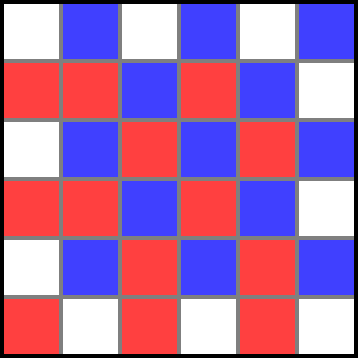
\includegraphics[width=0.45\textwidth]{FSI_6x6_DS.pdf}
    \hfill
    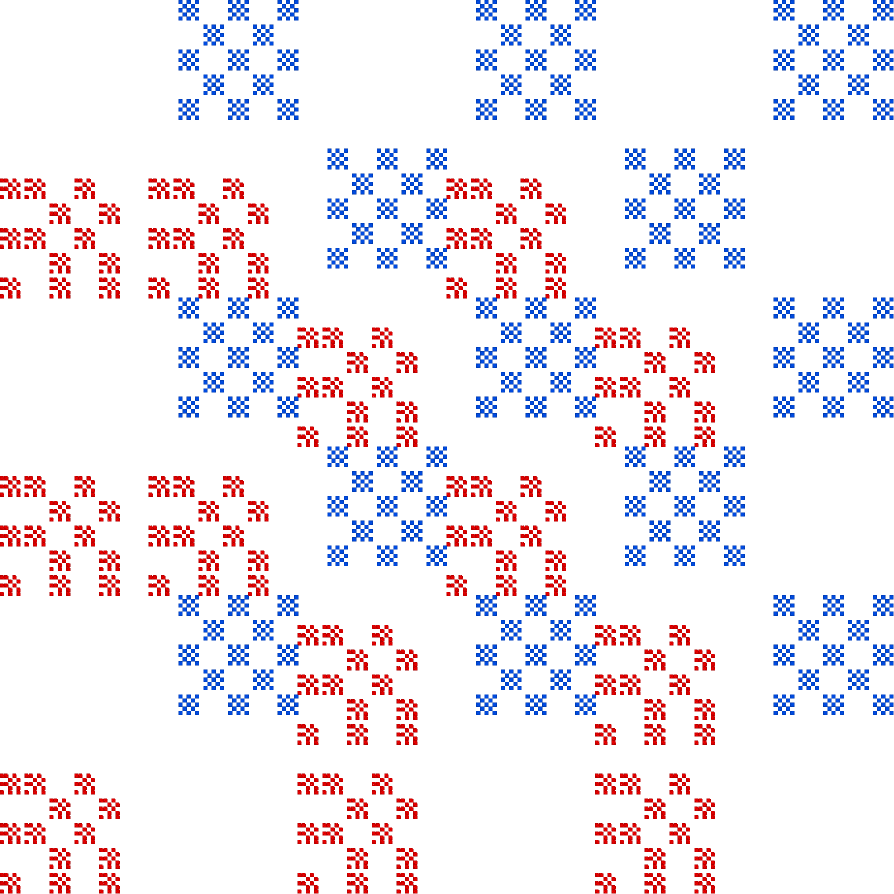
\includegraphics[width=0.45\textwidth]{FSI_6x6_K.png}
    \caption{Диаграмма множеств единиц для $D_1$ и $D_2$ (слева) и фрактальные квадраты $K_1$ и $K_2$ (справа).}
    % \label{fig:my_label}
\end{figure}


Множество $F_{(1,0)}$ пусто, поскольку $G_{(1,0)},F_{(1,1)}$ и $F_{(1,-1)}$ пусты. 
По той же причине $F_{(0,1)}=\0$. \\

Множества $G_{(-1,0)(-1,-1)}=\{(0,2),(0,4)\}$ и \\
$G_{0(-1,0)}=\{(1,2),(1,4),(2,3),(3,2),(3,4),(4,3)\}$.
Множества $G_{(0,-1)(-1,-1)}$ и $G_{0(0,-1)}$ получены их предыдущих двух.\\

Таким образом, после удаления пустых вершин и ребер
граф $\Ga_\Sa$ содержит четыре вершины  $F_0,F_{(-1,0)},F_{(0,-1)},F_{(-1,-1)}$ и четыре ребра, которым соответствуют $G_{(-1,0)(-1,-1)}, G_{(0,-1)(-1,-1)},G_{0(-1,0)}$ и $G_{0(0,-1)}$.

Вычисление с использованием формулы \eqref{perall} показывает, что
$\#F_{(-1,0)}=\#F_{(0,-1)}=2$ и $\#F_0=2 \#G_{0(-1,0)}+2\#G_{0(0,-1)}=24.$


\begin{figure}[H]
    \centering
    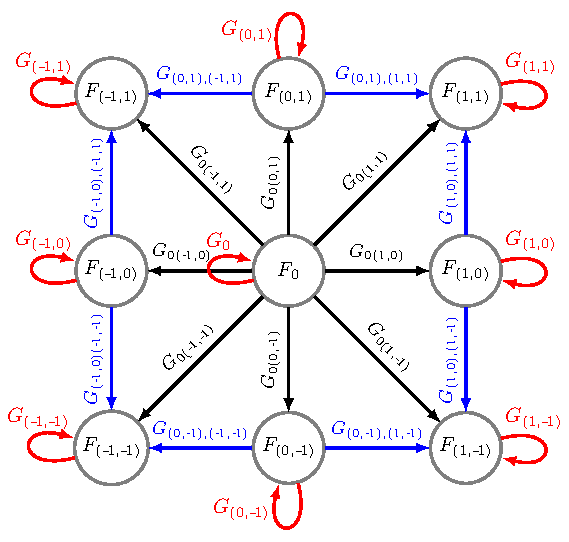
\includegraphics[width=.5\textwidth]{structure_grapg_full.pdf}
    \hfill
    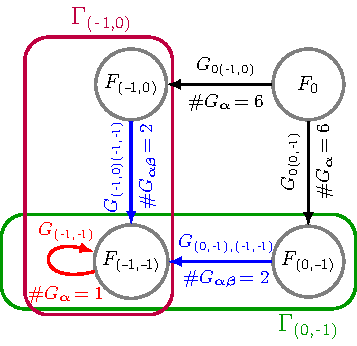
\includegraphics[width=.45\textwidth]{FSI_6x6_SG.pdf}
    \caption{Структурный граф $\Ga_\Sa$ в общем случае для пересечения двух фрактальных квадратов (слева) и сокращённый граф $\Ga_\Sa$ для Примера 1 (справа). На рисунке справа выделены подграфы $\Ga_{(-1,0)}$ и $\Ga_{(0,-1)}$. }
\end{figure} 
\end{example} 

\begin{example}
     
\end{example}

\subsection{Пересечения копий фрактального куба $K$.}

В случае, когда $K_1=K_2=K$, множества $F_\bma$ становятся пересечениями противоположных граней $K_\bma$ и $K_{-\bma}$ одного и того же фрактального куба $K$.
Если $\bma=0$, то $F_0=K$, в противном случае $F_\bma=F_{-\bma}$ для любого $\bma\neq 0$. 
Прямое вычисление показывает, что для любого $\bma$ верно $D_\bma=D\cap(D+(n-1)\bma)$ (подразумевая, что $D_{-\bma}=D_\bma-(n-1)\bma$).
Аналогично, $D_{-\bma-\bmb}=D\cap(D-n\bma+\bmb)=D_{\bma\bmb}-n\bma+\bmb$.


\subsection{Условие конечности меры $H^s(F_\al)$.}

\begin{definition}\label{nubma}
Для каждого $\bma\in A_k$ обозначим  $\nu(\bma)=\max\{\#G_\bmb : \bmb\succcurlyeq\bma\}$ и $s(\bma)=\log_n\nu(\bma)$.   
\end{definition}

Благодаря Замечанию \ref{qbma} мы также можем написать
$s(\bma)=\max\limits_{\bmb\succcurlyeq\bma}\{\dim_HQ_\bmb \}$.

\begin{theorem}\label{dimthm}
Для любого $\bma\in A_k$ размерность Хаусдорфа множества $F_\bma$ равна $s(\bma)$, а его $s(\bma)$-мера $H^{s(\bma)}(F_\bma)$ положительна.\\
Мера $H^{s(\bma)}(F_\bma)$ конечна тогда и только тогда, когда множество $\{\bmb\succcurlyeq\bma : \#G_\bmb=\nu(\bma)\}$ не содержит $\Ga$-сравнимых элементов.
\end{theorem}

\begin{proof}
Если мы возьмем $B=\bigcup\limits_{\bmb\succ\bma}T_{\bma\bmb}(F_\bmb)$, то Формула \eqref{perall} примет вид 
\begin{equation}
F_\bma=T_{\bma\bma}(F_\bma)\cup B.
\end{equation}

Повторяя последнюю формулу и имея в виду, что $\lim\limits_{m\to\8}T^m_{\bma\bma}(F_\bma)=Q_\bma$, мы получаем, что
\begin{equation}\label{FviaB}
F_\bma=Q_\bma\cup \bigcup\limits_{m=0}^\8T_{\bma\bma}^m(B)   
\end{equation}

Это равенство означает, что $\dim_HF_\bma=\max(\dim_HQ_\bma,\dim_HB)$.
Все невырожденные операторы $T_{\bma\bmb}$ сохраняют размерность, то есть $\dim_H T_{\bma\bmb}(F_\bmb)=\dim_H F_\bmb$. 
Из этого следует, что
$\dim_HB=\max\limits_{\bmb\succ\bma}\dim_HF_\bmb$, следовательно 
$\dim_HF_\bma=\max(\dim_HQ_\bma,\max\limits_{\bmb\succ\bma}\dim_HF_\bmb)$.

Предположим теперь, что $\dim_HF_\bma=s'>s(\bma)$.
Тогда $\dim_HB = s'$, следовательно, существует $\bmb\succ\bma$ такое, что $\dim_HF_\bmb=s'$.
Применяя этот аргумент к множеству $F_\bmb$, мы видим, что множество всех $\bmb\succ\bma$ таких, что $\dim_HF_\bmb=s'$, не может содержать минимальный элемент.
Однако это невозможно, потому что оно конечно.

Следовательно, $\dim_HF_\bma=s(\bma)$. \\

Если $\bmb\succ\bma$ и $\#G_\bmb=\nu(\bma)$, то
мера $H^{s(\bma)}(Q_\bmb)$ является положительной, следовательно мера $H^{s(\bma)}(F_\bma)$ тоже положительна.

Если $\#G_\bma>\#G_\bmb$ для любого $\bmb\succ\bma$, то $H^s(Q_\bmb)=0$ для всех
$\bmb\succ\bma$, следовательно, мера $H^s (F_\bma)=H^s (Q_\bma)$ конечна и положительна.\\
На этом завершается доказательство первого утверждения теоремы \ref{dimthm}.\\

Предположим теперь, что $\#G_\bma<\nu(\bma)$ и $H^s(B)=h>0$.
Тогда $H^s(T^m_\bma(B))=\dfrac{(\#G_\bma)^m h}{\nu(\bma)^m}$.
Беря сумму по всем $m$ от $0$ до $\8$, мы получаем $H^s(F_\bma)\leq \dfrac{h\nu(\bma)}{\nu(\bma)-\#G_\bma}$, следовательно, vthf $H^s(F_\bma)$ является положительной и конечной.\\

Теперь остается показать, что если для некоторого $\bmb\succ\bma$ мы имеем $\#G_\bmb=\#G_\bma=\nu(\al)$, то $H^s(F_\bma)$ бесконечно.
Это будет доказано в следующей лемме, которая завершает доказательство теоремы.\\
\end{proof}

Рассматривая Предложение \ref{falfa} и Замечание \ref{galfa}, нам достаточно рассмотреть ситуацию, когда $\bma=0$.


\begin{lemma}
Если $\#G_0=\#G_\bma=l$, $\log_nl=s$ и для любого $\bmb\succ 0$ верно $\#G_\bmb\le l$, то $H^s(F_0)$ бесконечна.
\end{lemma}

\begin{proof} 
{\bf Случай 1}: Существует $d_1\in D_1$ такое, что $d_1+\bma\in D_2$.\\

Рассмотрим фрактальные кубы $Q_0$ и $Q_\bma$ и отметим, что оба множества $Q_0$ и $Q_\bma$ имеют конечную положительную меру в размерности $s$.

Рассмотрим множество $Q_*$, определяемое уравнением \\
$Q_*= \dfrac{Q_*+G_0}n\bigcup\dfrac{d_1+Q_\bma}n$.
Определим оператор $T_0$ равенством $T_0(A)= \dfrac{A+G_0}n$. 
Пусть $B=\dfrac{d_1+Q_\bma}n$.
 
Пусть $\hT$ --- оператор, определяемый равенством $\hT(A)= \dfrac {I^k+A}n$, аттрактором которого является весь куб $P$.

Рассмотрим множества $P_\bma^{(m)}=\hT^m(P_\bma)$.
Включение $P_\bma\IN\hT(P_\bma)$ означает, что эти множества образуют возрастающую вложенную последовательность $P_\bma\IN P_\bma^{(1)}\IN P_\bma^{(2)}\ldots$.

Заметим, что $B\IN P_\bma^{(1)}\mmm P_\bma$ и $T_0^m(B)\IN \hT^m(B)\IN P_\bma^{(m+1)}\mmm P_\bma^{(m)}$.
Множества $P_\bma^{(m+1)}\mmm P_\bma^{(m)}$ не пересекаются, следовательно, множества $T_0^m(B)$ тоже не пересекаются.

С другой стороны, поскольку $\#G_0=\#G_\bma=l$, $H^ s(T_0^m(B))=H^s(B)$.
Следовательно, множество $\bigcup\limits_{m=0}^\8 T_0^m(B)$ имеет бесконечную меру Хаусдорфа в размерности $s$.\\
 
{\bf Случай 2.}   
Существует последовательность $0\prec\bma_1\prec\ldots\prec\bma_{p}$ такая, что $\bma_p=\bma$ и $\#G_{0\bma_1}\#G_{\bma_1\bma_2}\ldots\#G_{\bma_{p-1}\bma_p}\neq 0$.
Тогда для каждого $i\in\{1,\ldots,p\}$ существует $d_i\in D_1$ и  $\da_i\in D_2$ such that $\da_i=d_i-n\bma_{i-1}+\bma_i$.
Тогда \[\sum\limits_{i=1}^p n^{p-i}\da_i=\sum\limits_{i=1}^p n^{p-i}(d_i-n\bma_{i-1}+\bma_i)=\sum\limits_{i=1}^p n^{p-i} d_i +\bma_p.\] 
То есть $\bm{\da}_{i_1\ldots i_p}-\bm{d}_{i_1\ldots  i_p}=\bma_p$.
 
Это означает, что если мы рассмотрим $K_1$ и $K_2$ как фрактальные кубы порядка $n^p$ с множествами единиц $D_1^ {(p)}$ и $D_2^{(p)}$ соответственно, то множество $G^{(p)}_{0\bma}$ непусто.
В то же время равенства $D^{(p)}_{1,\bma}= D^{(p)}_1\cap(n^p-1)P_\bma=(D_{1,\bma})^{(p)}$ и $D^{(p)}_{2,-\bma}= D^{(p)}_2\cap(n^p-1)P_{-\bma}=(D_{2,-\bma})^{(p)}$ означают, что  $G^{(p)}_\bma=(G_\bma)^{(p)}$. 
Из этого следует, что $\#G^{(p)}_\bma=l^p$ и $\log_{n^p}\#G^{(p)}=s$.
Следовательно, фрактальный куб порядка $n^p$ с множеством единиц $G^{(p)}_\bma$ совпадает с $Q_\bma$.
  
Эта ситуация совпадает со Случаем 1, следовательно, мера $H^s(F_0)$ бесконечна.
\end{proof}

\begin{example}
На следующем Рисунке изображена пара фрактальных квадратов, $K_1$ и $K_2$ порядка $4$ и размерности $3/2$.
Поскольку множество $G_0$ состоит из $4$ элементов, пересечение $F_0$ имеет размерность, равную $1$.
Однако множество $G_{(0,-1)}$ также состоит из $4$ элементов, поэтому мера множества $F_0$ бесконечна.

\begin{figure}[H]
    \centering
    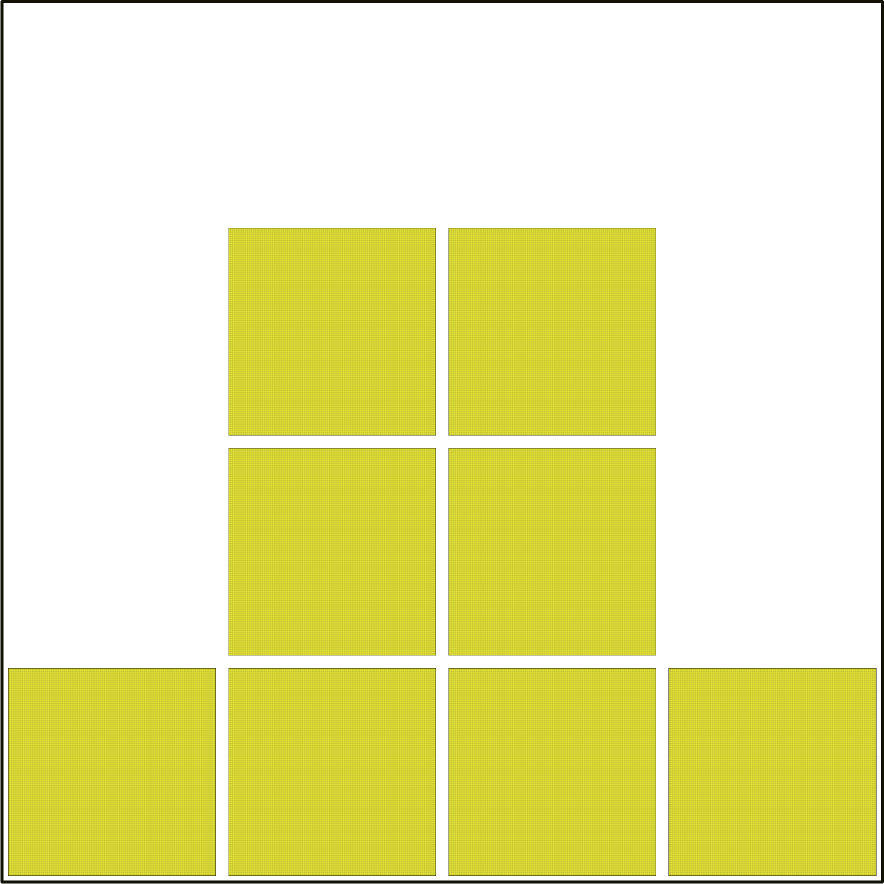
\includegraphics[width=0.22\textwidth]{e1P1.png} 
    \hfill
    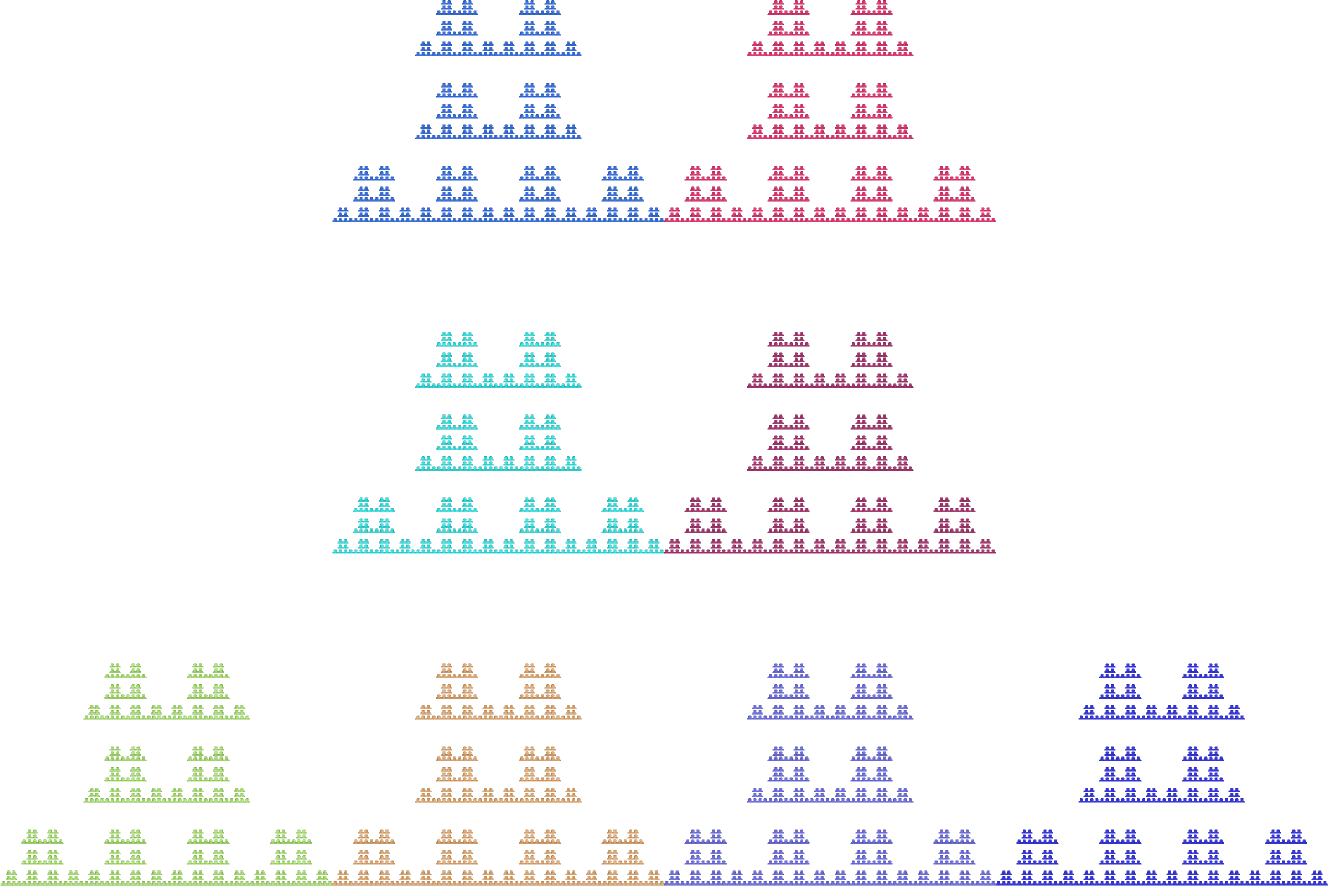
\includegraphics[width=0.22\textwidth]{e1K1.png} 
    \hfill
    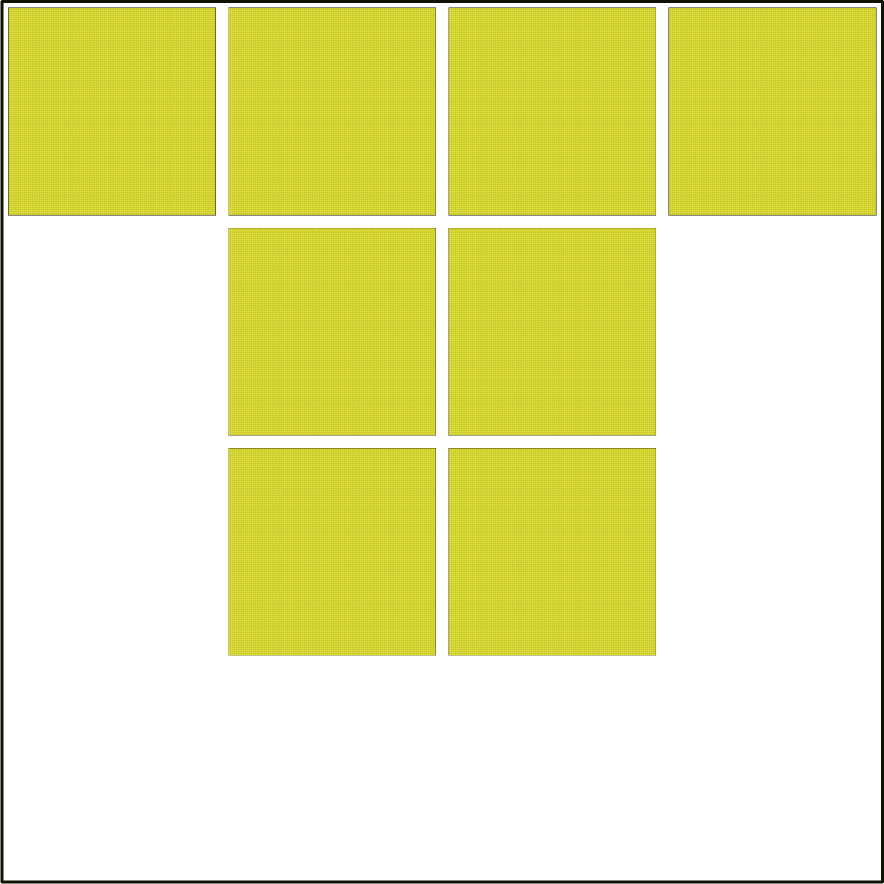
\includegraphics[width=0.22\textwidth]{e1P2.png} 
    \hfill
    \begin{minipage}[b][0.22\linewidth][t]{0.22\linewidth}
    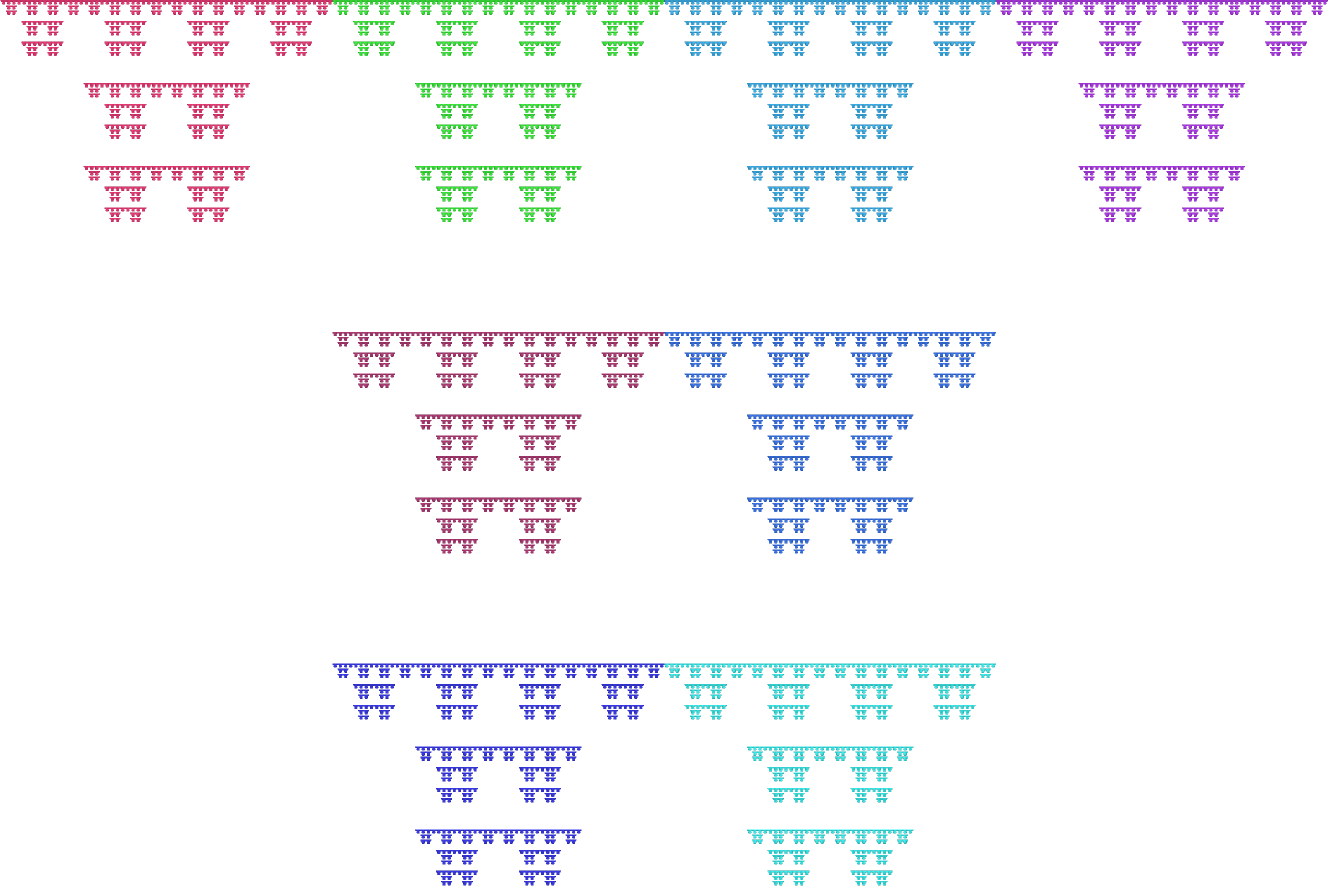
\includegraphics[width=\textwidth]{e1K2.png} 
    \end{minipage}
    \vfill\vspace{2mm}
    \hspace{1cm} $\dfrac{D_1+P}{n}$ \hfill $K_1=\dfrac{K_1+P}{n}$ \hfill $\dfrac{D_2+P}{n}$ \hfill $K_2=\dfrac{K_2+P}{n}$\hspace{1cm}
    \caption{}
    \label{fig:fs1and2}
\end{figure}

\begin{figure}[H]
    \centering
    \begin{minipage}[b][0.4\linewidth][c]{0.4\linewidth}
    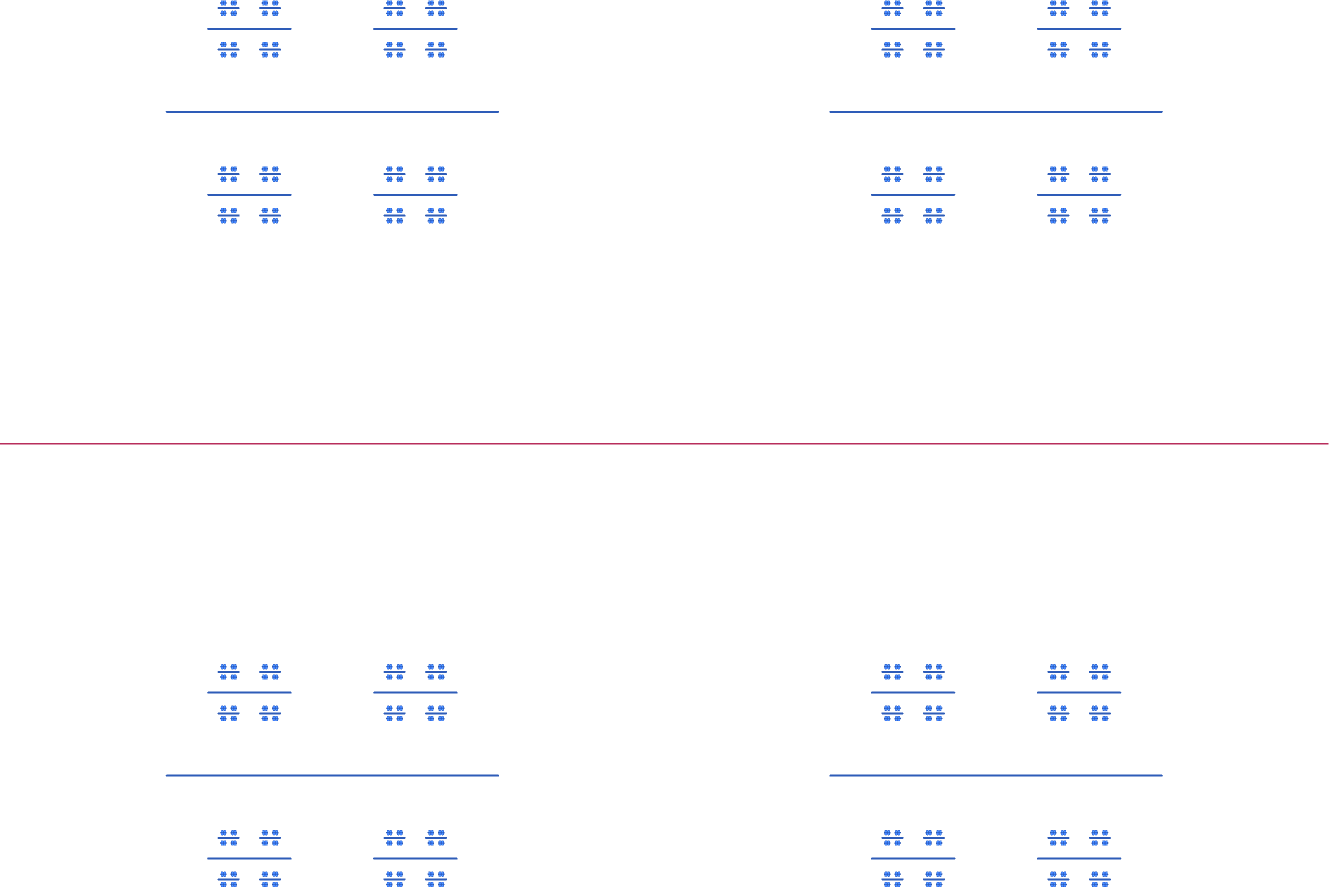
\includegraphics[width=\textwidth]{e1K12.png} 
    \end{minipage}
    \hfill
    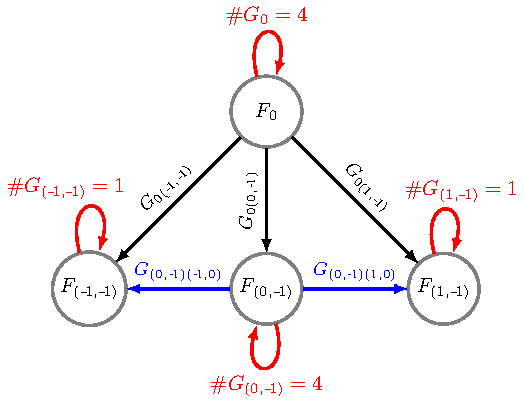
\includegraphics[width=0.56\textwidth]{sg_GDS_InfM.pdf} 
    \vfill\vspace{2mm}
    \hspace{2cm} $F_0=K_1\cap K_2$ \hfill $\Gamma(K_1,K_2)$\hspace{3.5cm}
    \caption{}
    \label{fig:fs_int}
\end{figure}

\end{example}


\subsection{Мощность множества $F_\al$.}

\begin{theorem}\qquad
\begin{enumerate}[nolistsep]
\item Множество $F_\bma$ является одноточечным, если $\Gamma_\bma$ представляет собой цепочку $\bma=\bma_1\prec\ldots\prec\bma_p$, в которой для всех $j\le p-1$, $\# G_{\bma_j\bma_{j+1}}=1$, $G_{\bma_j}=\0$ и $\#G_{\bma_p}=1$;
\item Множество $F_\bma$ конечно, если для всех максимальных вершин $\bmb$ в $\Gamma_\bma$, верно $\#G_\bmb=1$ и $G_{\bmb}=\0$ для всех остальных вершин в $\Gamma_\bma$.
В этом случае $\#F_\bma$ равно сумме всех композиций $\prod \limits_{j=1}^{p-1}\# G_{\bma_j\bma_{j+1}}$, взятых по всем цепочкам $\bma=\bma_1\prec\ldots\prec\bma_p=\bmb$, где $\bmb$ является максимальным в $\Gamma_\bma$;
\item Множество $F_\bma$ счетно, если $\#G_\bmb\le 1$ для всех вершин $\bmb$ в $\Gamma_\bma$;
\item Множество $F_\bma$ несчетно, если в $\Gamma_\bma$ существует такая вершина $\bmb$, что $\#G_\bmb> 1$.
\end{enumerate}
\end{theorem}

\begin{corollary}
Фрактальный куб $K$ обладает свойством одноточечного пересечения, если структурный граф $\Gamma(\Sa)$ представляет собой объединение цепочек $0\prec\bma_{i1}\prec\ldots\prec\bma_{ip_i}$, для которых все $\bma_{ij}$ различны и таковы, что для всех $i$ верно $\#G_{\bma_{ip_i}}=1$ и для всех $i,j$ таких, что $j\le p_i-1$, верно $\# G_{\bma_{ij}\bma_{i,j+1}}=1$ и $G_{\bma_{ij}}=\0$.

Фрактальный куб $K$ обладает свойством конечного пересечения, если для всех максимальных $\bma$ в графе $\Ga (\Sa)$, $\#G_\bma=1$ и для всех остальных $\bma\neq 0$, $\#G_\bma=0$.
\end{corollary}

\begin{example}[Фрактальный куб с одноточечным пересечением]
Возьмем фрактальный куб $K=\dfrac{K+D}{4}$ с множеством единиц 
\begin{equation*}
\begin{split}
D=\{
    &(0,0,0), (1,1,1), (2,2,2), (3,3,3), (2,1,1), (1,2,1), (1,1,2), (1,2,2),\\ 
    &(2,2,1), (2,1,2), (0,0,2), (0,2,1), (3,3,1), (3,1,1), (2,0,0), (1,2,0),\\ 
    &(1,3,3), (1,1,3)\}     
\end{split}
\end{equation*}
 
\begin{figure}[H]
    \centering
    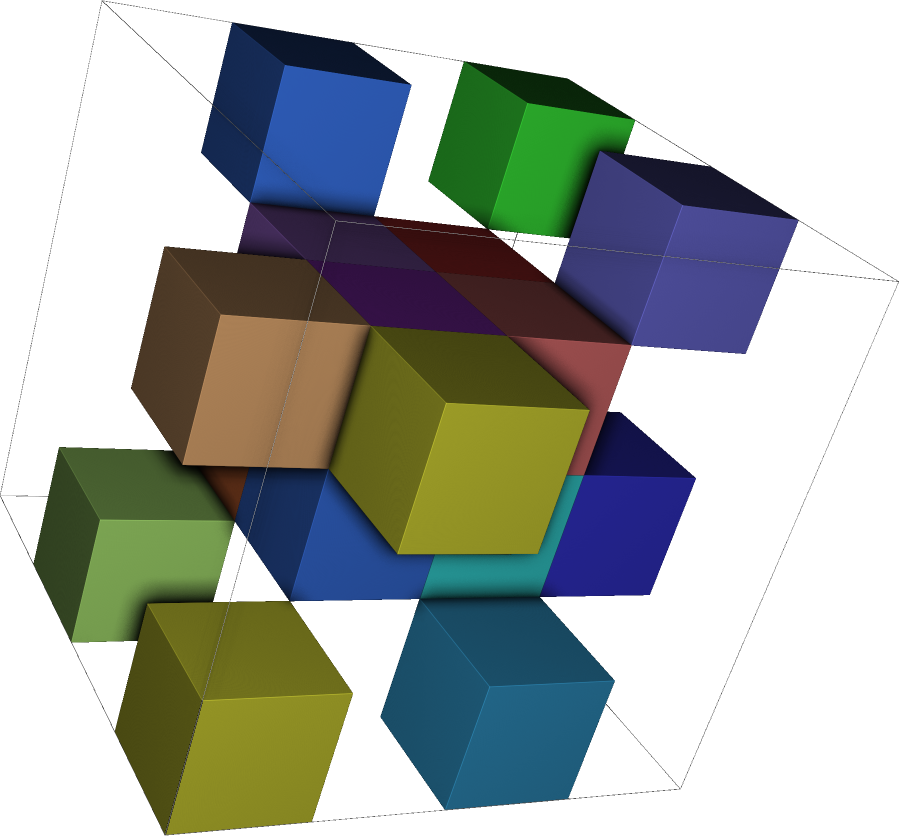
\includegraphics[width=0.45\textwidth]{fqP1a.png}
    \hfill
    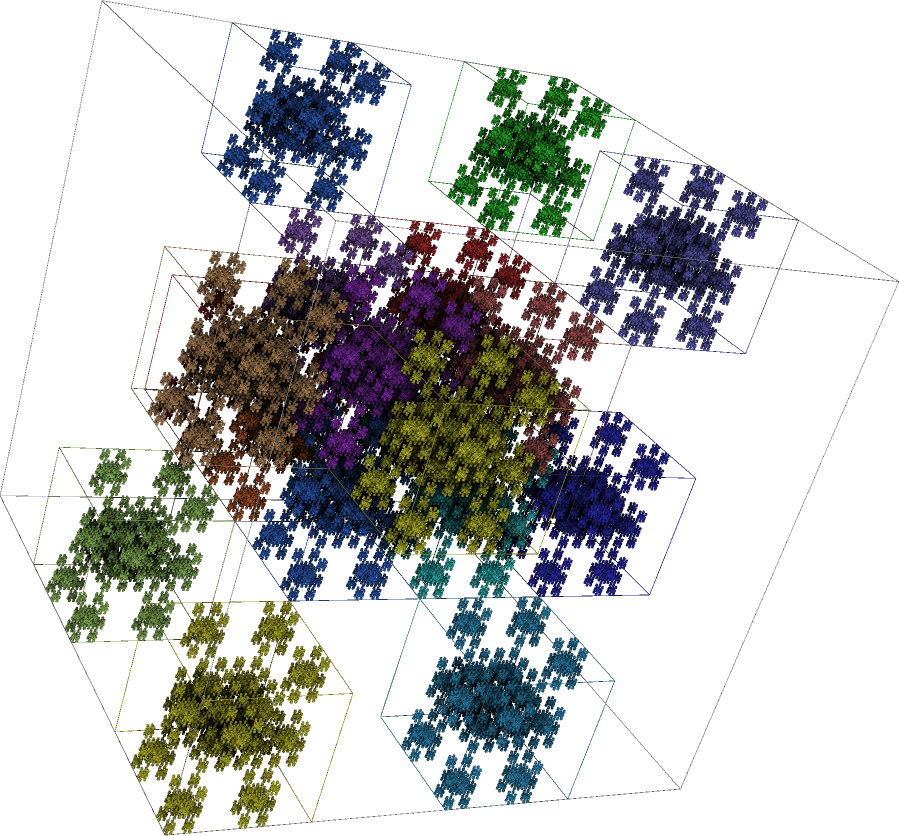
\includegraphics[width=0.45\textwidth]{fqK1a.png}
    \caption{Фрактальный куб с одноточечным пересечением}
    \label{fig:fq}
\end{figure}

\begin{figure}[H]
    \centering
    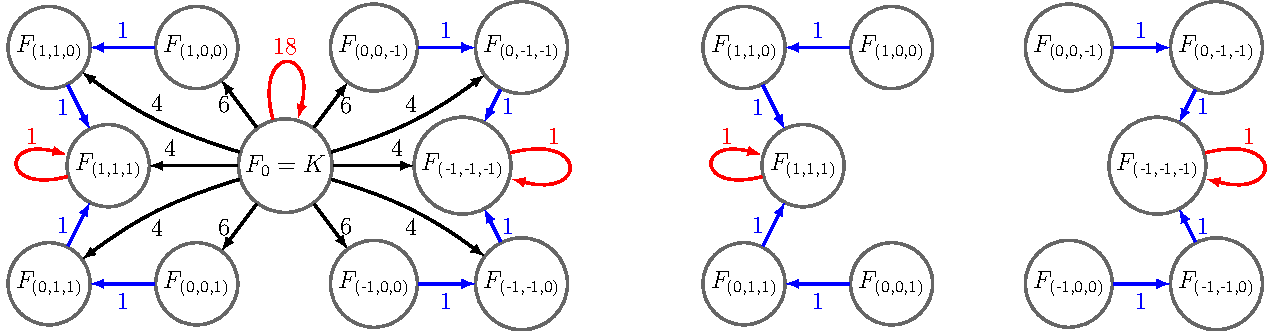
\includegraphics[width=\textwidth]{SG_for_FQ.pdf}
    \caption{Структурный граф}
    \label{fig:fq_sg}
\end{figure}
\end{example}

\begin{figure}[H]
    \centering
    \hfill
    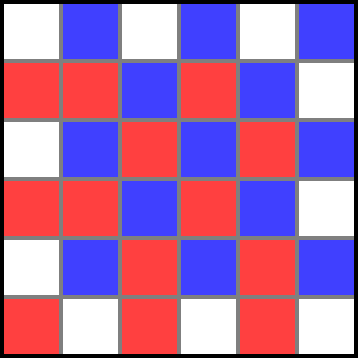
\includegraphics[width=0.45\textwidth]{FSI_6x6_DS.pdf}
    \hfill
    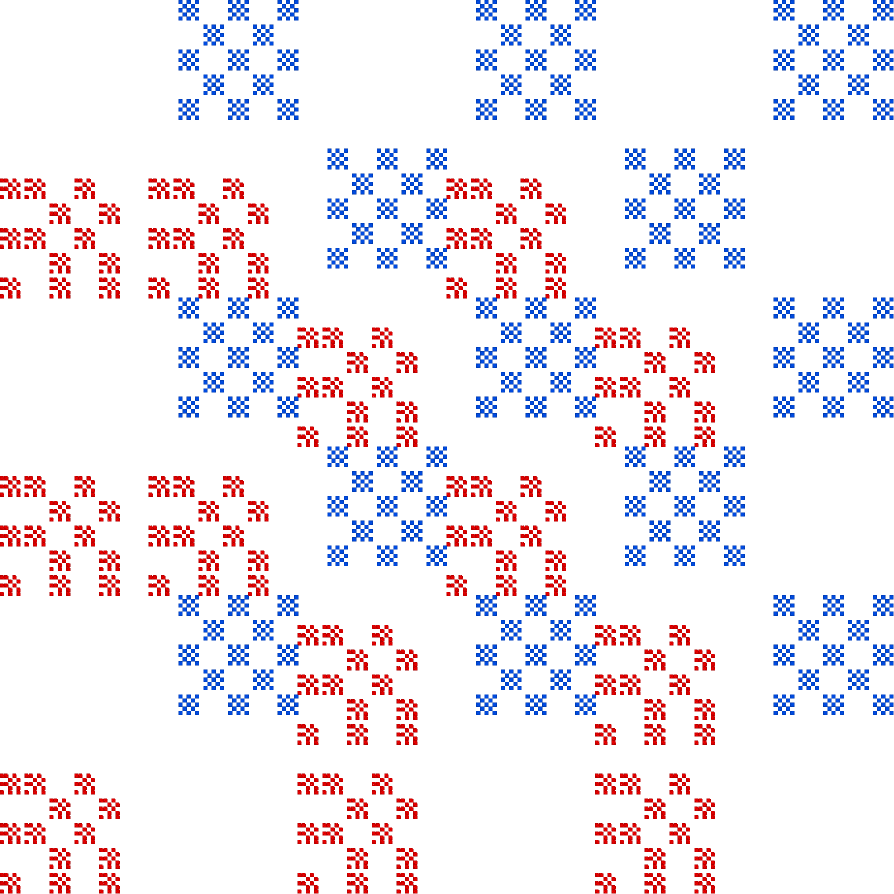
\includegraphics[width=0.45\textwidth]{FSI_6x6_K.png}
    \hfill
    \caption{Пересечение фрактальных квадратов по 24 точкам}
    \label{fig:FSI_6x6}
\end{figure}

\begin{example}[Пересечение по 24 точкам]
\label{ex:FSI_6x6}
На Рисунке \ref{fig:FSI_6x6} представлено пересечение двух фрактальных квадратов $K_1$ и $K_2$ порядка $6$ (синее и красное множество), а на Рисунке \ref{fig:FSI_SG} слева показан структурный граф $\Gamma_{\Sigma(K_1,K_2)}$ этого пересечения.
По этому графу легко понять, что пересечение $F_0$ конечно, причем $\#F_0=24.$
\end{example}

\begin{figure}[H]
    \centering
    \hfill
    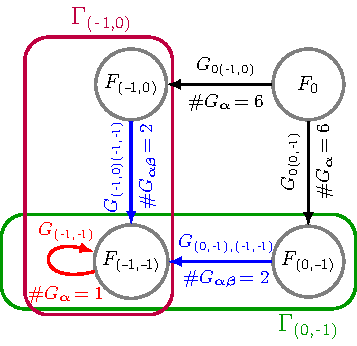
\includegraphics[width=0.35\textwidth]{FSI_6x6_SG.pdf}
    \hfill
    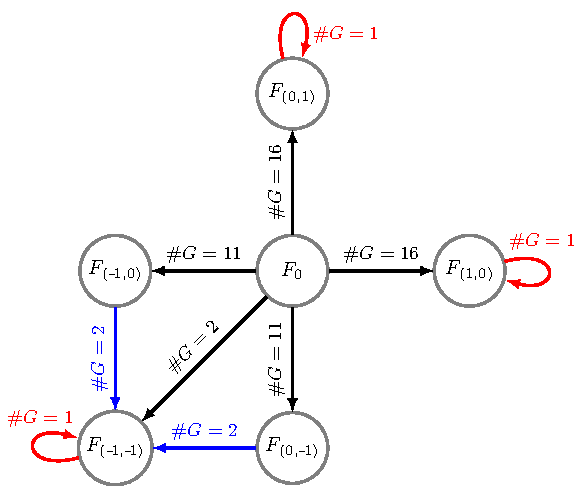
\includegraphics[width=0.55\textwidth]{FSI_7x7_SG.pdf}
    \hfill
    \caption{Структурные графы пересечений на рисунках \ref{fig:FSI_6x6} и \ref{fig:FSI_7x7}}
    \label{fig:FSI_SG}
\end{figure}

\begin{example}[Пересечение по 78 точкам]
\label{ex:FSI_6x6}
На Рисунке \ref{fig:FSI_7x7} представлено пересечение двух фрактальных квадратов $K_1$ и $K_2$ порядка $7$ (синее и красное множество), а на Рисунке \ref{fig:FSI_SG} справа показан структурный граф $\Gamma_{\Sigma(K_1,K_2)}$ этого пересечения.
По этому графу,аналогично предыдущему примеру, легко понять, что $\#F_0=78.$

\end{example}

\begin{figure}[H]
    \centering
    \hfill
    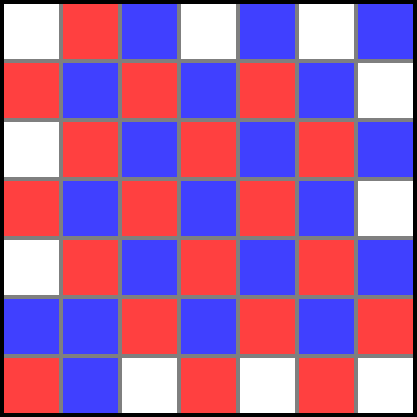
\includegraphics[width=0.45\textwidth]{FSI_7x7_DS.pdf}
    \hfill
    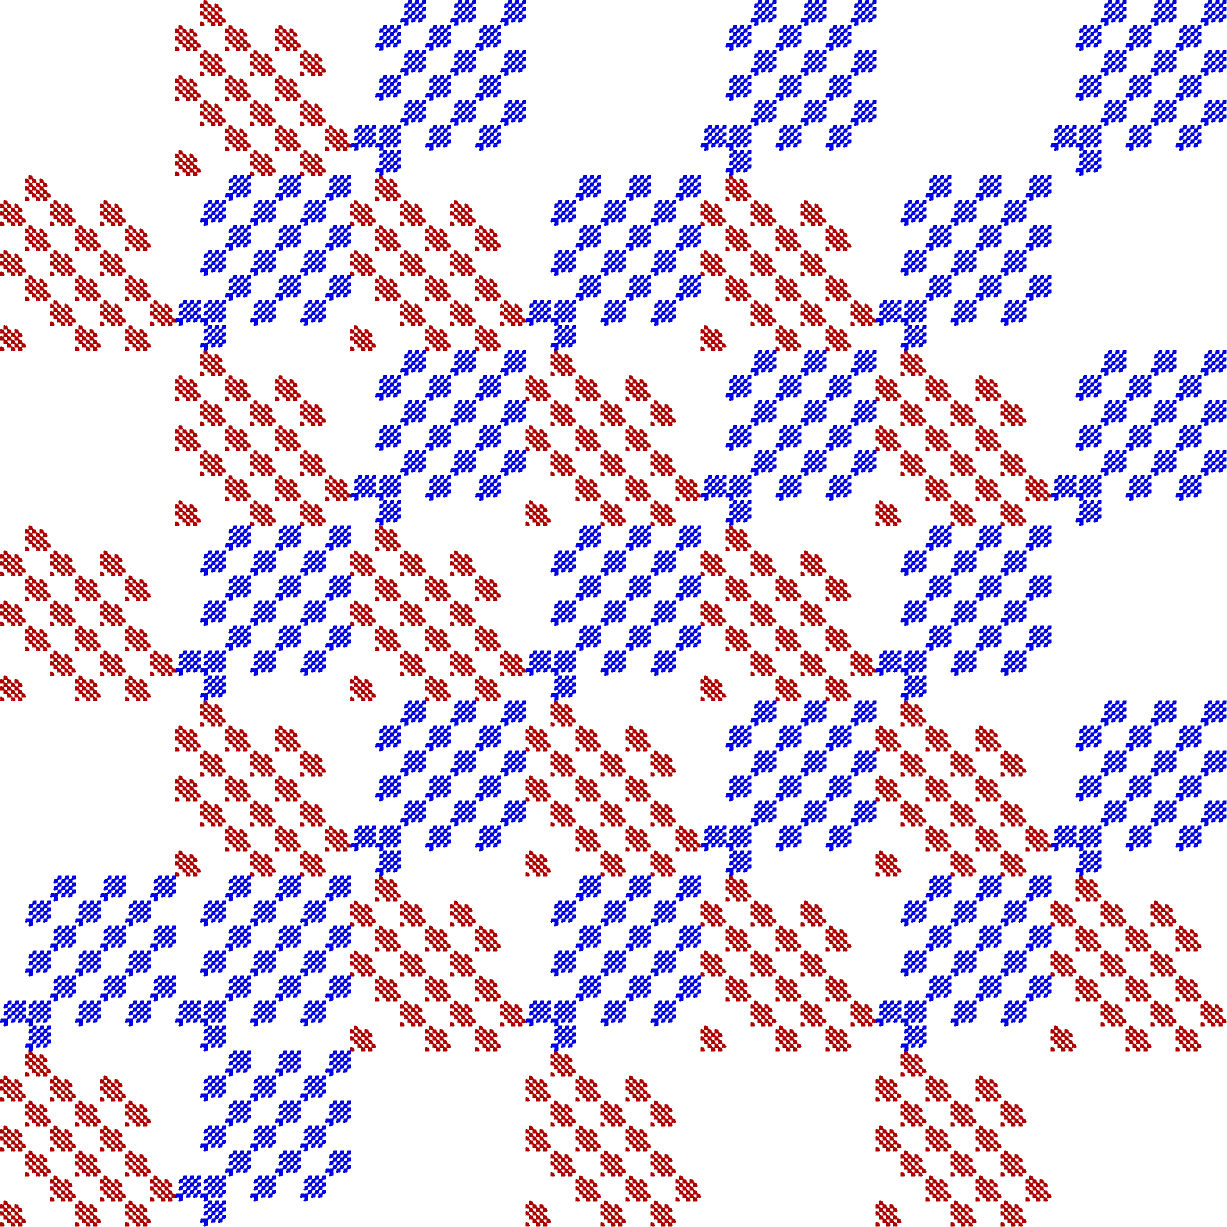
\includegraphics[width=0.45\textwidth]{FSI_7x7_K.png}
    \hfill
    \caption{Пересечение фрактальных квадратов по 78 точкам}
    \label{fig:FSI_7x7}
\end{figure}


\section{Дендритность фрактального куба}

В этом параграфе рассмотрим фрактальные кубы (с одноточечным пересечением) и проверим, является ли рассматриваемое множество дендритом.
Метод определения свойства дендритности фрактального куба основан на нахождении двудольного графа пересечений фрактального куба.

\subsection{Свойство одноточечного пересечения и критерий дендритности}

\begin{definition}\label{fipss}\cite{FIP}
Система множеств с одноточечным пересечением (было в главе 1)  
\end{definition}

\begin{definition}\label{fipcs}
Система сжимающих подобий со свойством одноточечного пересечения.(было в главе 1)
\end{definition}

\subsection{Алгоритм проверки фрактального куба на свойство дендритности}

Пусть $K$ --- фрактальный $k$-куб.
Чтобы проверить $K$ на наличие дендритности, нужно выполнить следующие шаги:

 \begin{enumerate}

    \item Найдём все множества $G_\bma, G_{\bma\bmb}$ для системы $\Sigma=\Sigma(K,K)$ и запишем систему $\Sa$.
    Согласно Определению \ref{strg} и Лемме \ref{red}, исключим все исчезающие вершины и ребра и построим граф $\Ga_\Sa$.
   
    \item Используя Следствие \ref{SIPQ}, проверим выполнение свойства одноточечного пересечения для $K$.
    Если это не удается, то $K$ не является дендритом.
    
    \item Построим двудольный граф пересечений для фрактального куба $K$, соединив рёбрами пересекающиеся копии с точкой пересечения этих копий. 
    Нужно учесть случай с кратными точками, упомянутыми в следствии \ref{mpoint}.
    Теперь если получившийся двудольный граф пересечений будет деревом, то $K$ --- дендрит.
    
\end{enumerate}